\documentclass[10pt,twocolumn,letterpaper]{article}
\usepackage{graphicx}
\usepackage{placeins}
\usepackage{float}
\usepackage{subfigure}
\usepackage{gensymb}
\usepackage{url}
\usepackage{hyperref}
%\usepackage[table]{xcolor} 
\usepackage{times}
\usepackage{color}
%\usepackage{multirow} %mk
\usepackage{verbatim}

\usepackage{multirow}

\begin{document}

\begin{figure*}[th]
{\small{
\begin{center}
\begin{tabular}{@{}c@{\,\,\,}c@{\,\,\,}c@{\,\,\,}c@{\,\,\,}c@{\,\,\,}}
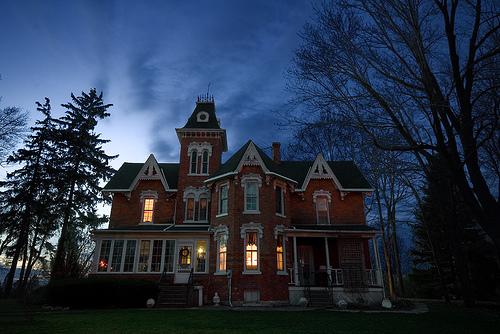
\includegraphics[width=0.19\textwidth]{imggrid/falseposi/1.jpg} &
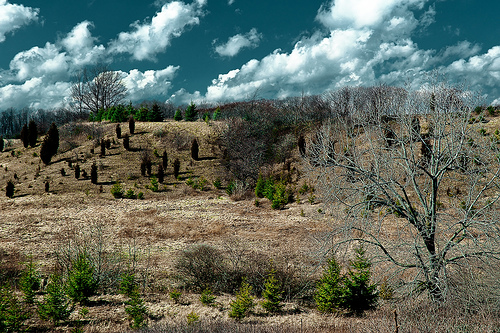
\includegraphics[width=0.19\textwidth]{imggrid/falseposi/2.jpg} &
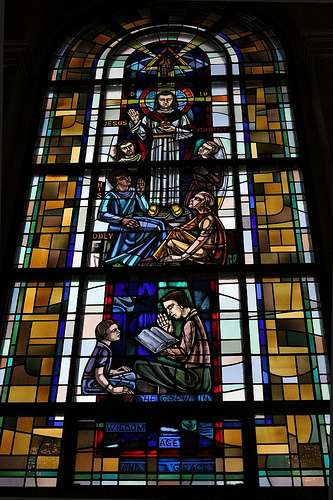
\includegraphics[height=1in]{imggrid/falseposi/3.jpg} &
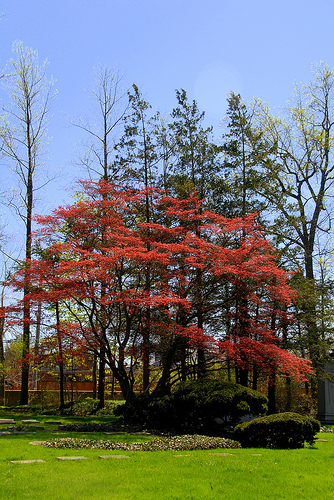
\includegraphics[height=1in]{imggrid/falseposi/4.jpg} &
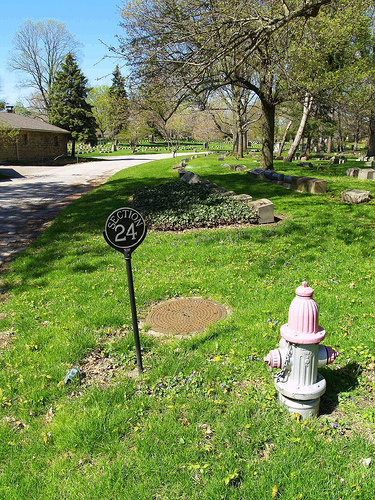
\includegraphics[height=1in]{imggrid/falseposi/5.jpg} \\
%\multicolumn{5}{c}{(a) Random positive images in vegetation dataset} \\
\\[-6pt]
\hline
\\[-6pt]
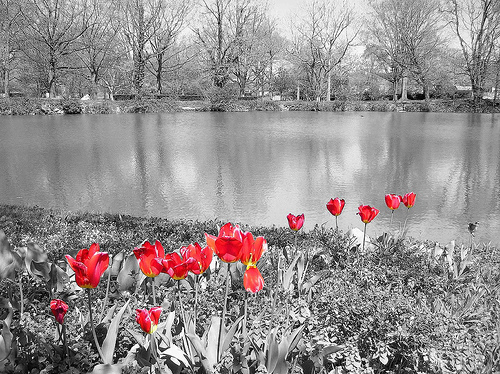
\includegraphics[width=0.19\textwidth]{imggrid/falseposi/6.jpg} &
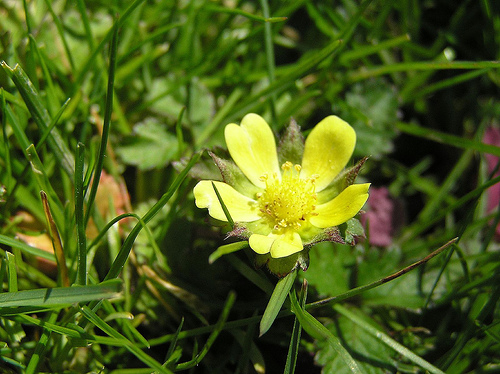
\includegraphics[width=0.19\textwidth]{imggrid/falseposi/7.jpg} &
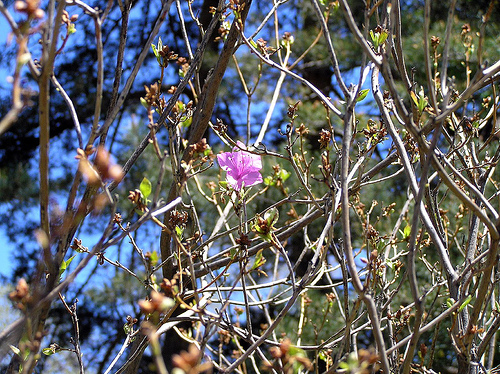
\includegraphics[width=0.19\textwidth]{imggrid/falseposi/8.jpg} &
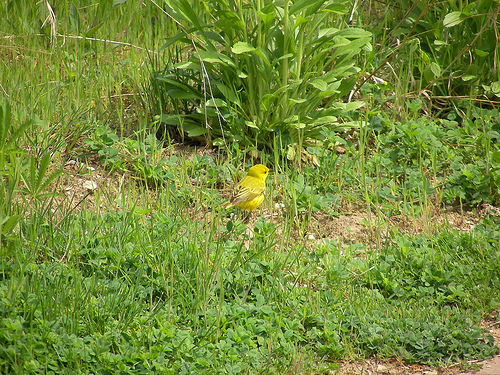
\includegraphics[width=0.19\textwidth]{imggrid/falseposi/9.jpg} &
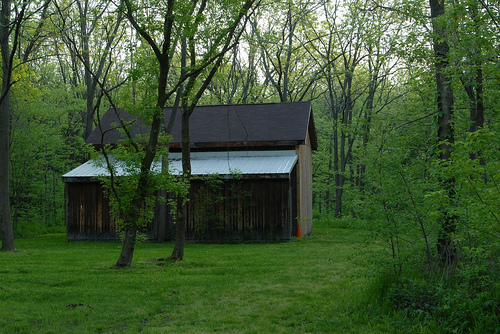
\includegraphics[width=0.19\textwidth]{imggrid/falseposi/10.jpg} \\
\multicolumn{5}{c}{(a) Random positive images in vegetation dataset} \\ 
\\[-6pt]
\hline
\\[-6pt]
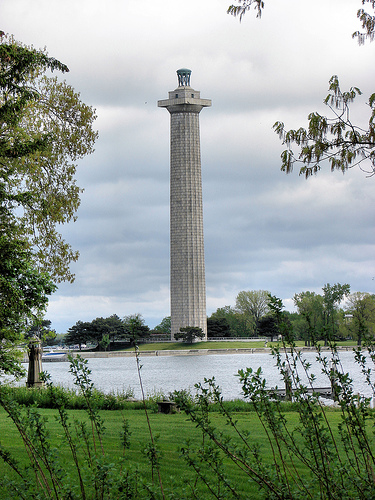
\includegraphics[height=1in]{imggrid/falseposi/11.jpg} &
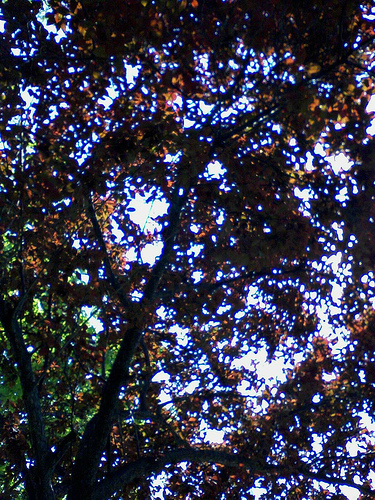
\includegraphics[height=1in]{imggrid/falseposi/12.jpg} &
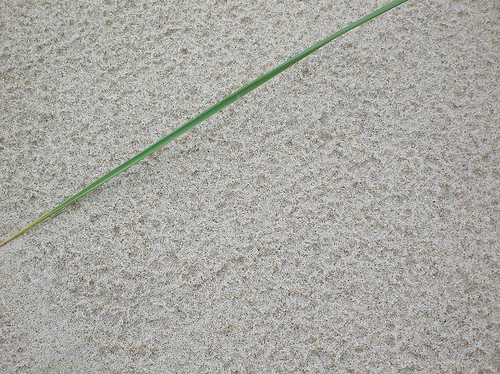
\includegraphics[width=0.19\textwidth]{imggrid/falseposi/13.jpg} &
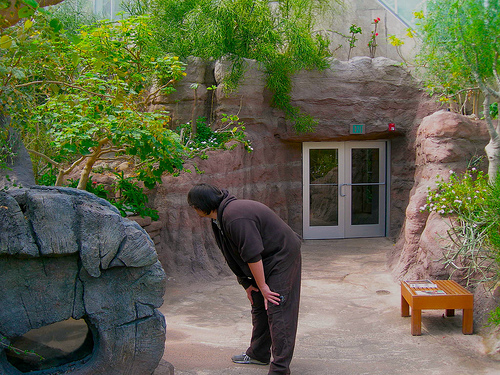
\includegraphics[width=0.19\textwidth]{imggrid/falseposi/14.jpg} &
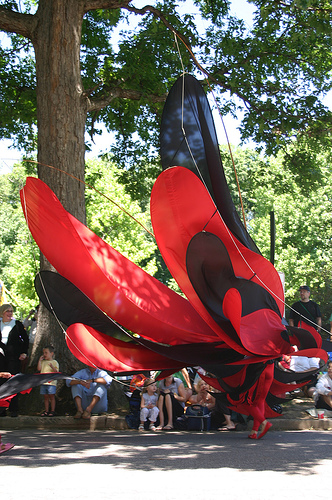
\includegraphics[height=1in]{imggrid/falseposi/15.jpg} \\
%\multicolumn{5}{c}{(c) Random false negatives (snow images classified as non-snow)} \\ 
\\[-6pt]
\hline
\\[-6pt]
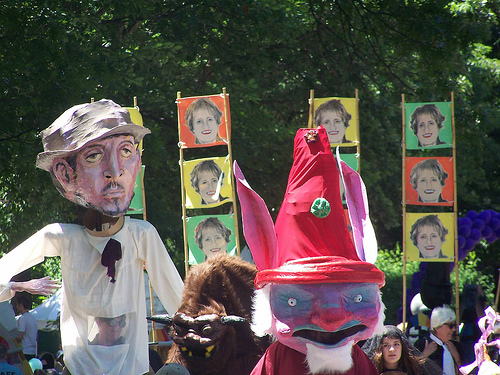
\includegraphics[width=0.19\textwidth]{imggrid/falseposi/16.jpg} &
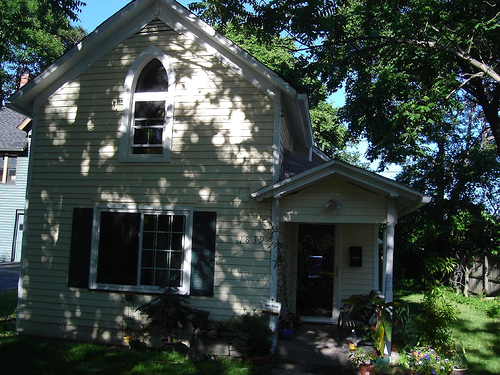
\includegraphics[width=0.19\textwidth]{imggrid/falseposi/17.jpg} &
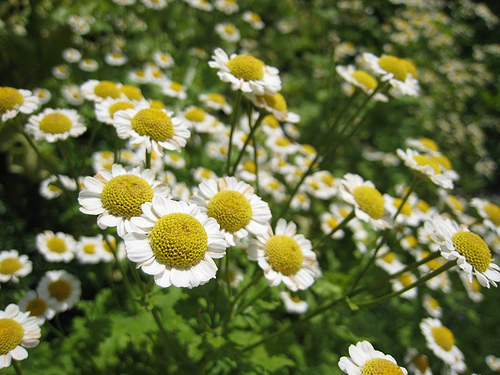
\includegraphics[width=0.19\textwidth]{imggrid/falseposi/18.jpg} &
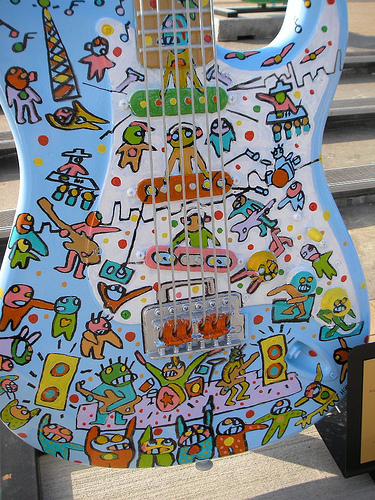
\includegraphics[height=1in]{imggrid/falseposi/19.jpg} &
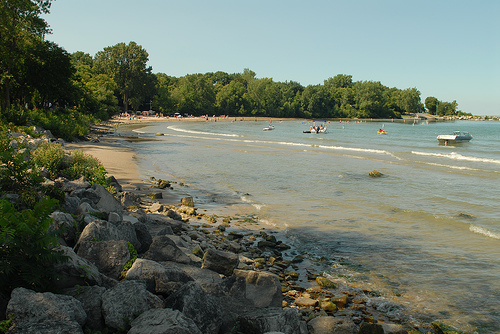
\includegraphics[width=0.19\textwidth]{imggrid/falseposi/20.jpg} \\
\multicolumn{5}{c}{(b) Random negative images in vegetation dataset} \\
\end{tabular}
\end{center}
}}
\caption{In all false positive bins, there are 47 images that are predicted as greenery. And these images are the reason these bins are predicted as green. Here are some random selected examples of the green images.}
\label{fig:falseposi}
\end{figure*}

% bar plot of 2 places
\begin{figure}
%{\small{
\begin{center}
\begin{tabular}{c c}
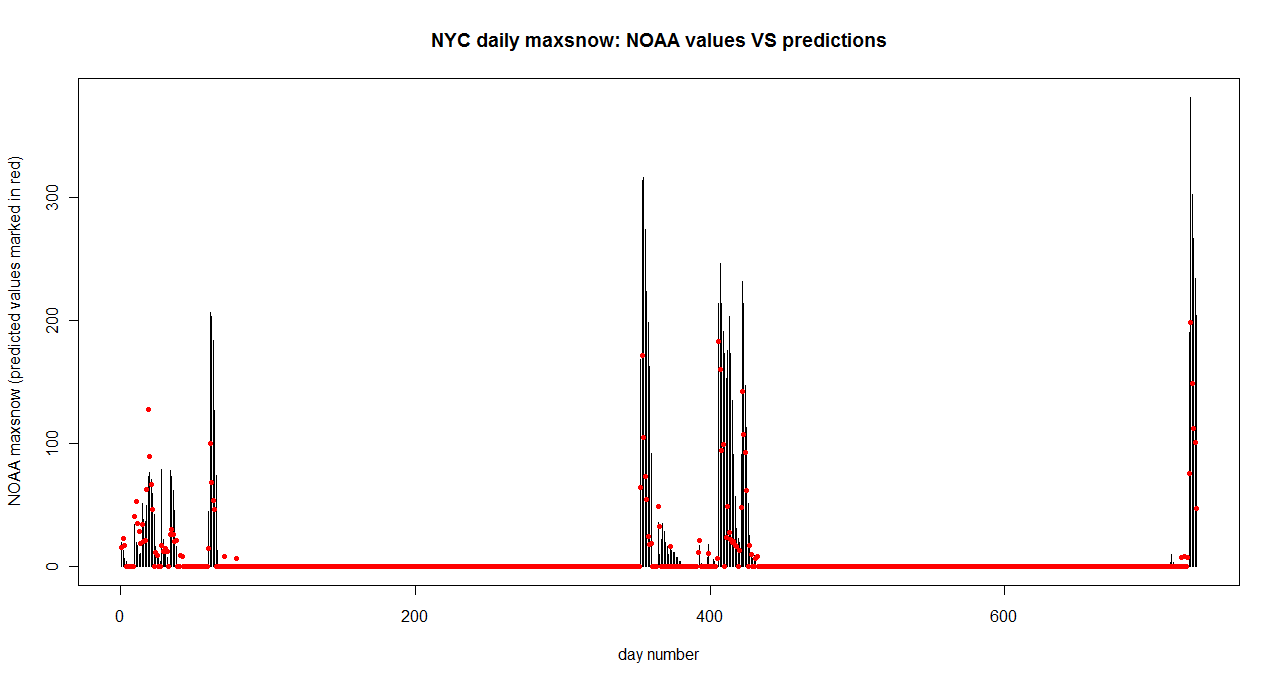
\includegraphics[width=0.22\textwidth]{plots/nyc_noaa_vs_prediction_prev_3.png} &
%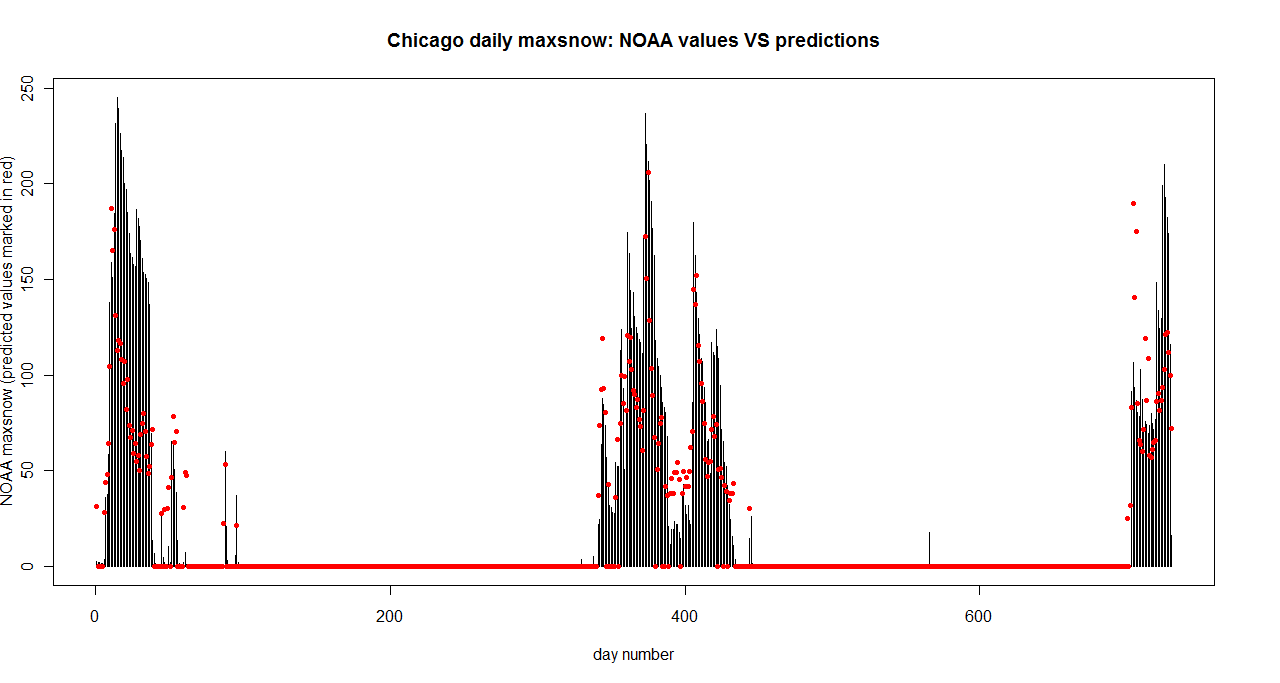
\includegraphics[width=0.5\textwidth,height=1.4in,clip,trim=0 0.5in 0in 0.6in]{plots/chicago_noaa_vs_prediction_prev_3.png} 
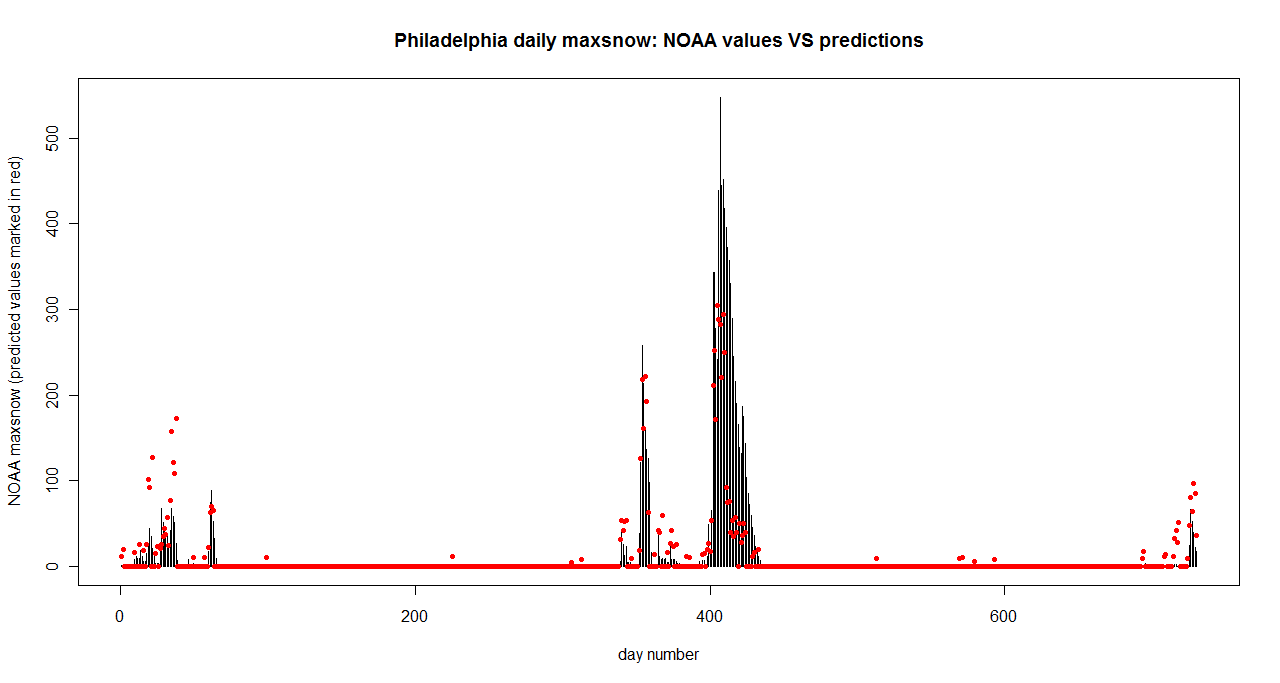
\includegraphics[width=0.22\textwidth]{plots/philly_noaa_vs_prediction_prev_3.png} \\
(a) & (b)\\
\end{tabular}
\end{center}
%}}
\vspace{-24pt}
\caption{Comparing time series of actual daily snowfall (in mm) for Chicago with estimates using Flickr, for Jan 2009--Dec 2010 and $T=3$. Red dots show predictions, and vertical bars show actual values.}
\label{fig:prediction_vis}
\vspace{-12pt}
\end{figure}

\begin{table}[b]
\begin{center}
{\footnotesize{
\begin{tabular}{|l|c|c|}
\hline 
--- & \multicolumn{2}{c|}{Ground truth}\tabularnewline
\hline
--- & Greenery & Not Greenery\tabularnewline
\hline 
\hline 
%Random Baseline  & --- & 50.0\%\tabularnewline
%\hline 
%\hline
Greenery & --- & ---\tabularnewline
\hline 
Not Greenery  & --- & ---\tabularnewline
\hline
\end{tabular}
}}
\caption{Confusion matrix of vegetation detection in 2007}
\label{tab:confusionmatrix}
\end{center}
\end{table}


\begin{figure*}[th]
{\small{
\begin{center}
\begin{tabular}{@{}c@{\,\,\,}c@{\,\,\,}c@{\,\,\,}c@{\,\,\,}c@{\,\,\,}}
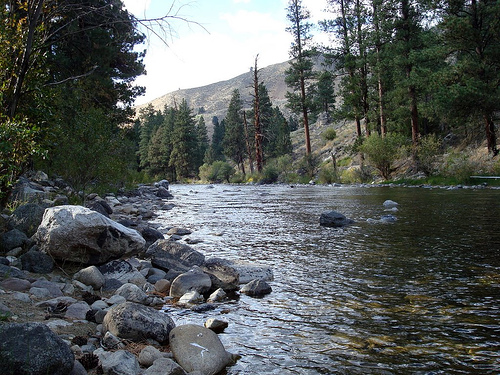
\includegraphics[width=0.19\textwidth]{imggrid/datasetposi/1.jpg} &
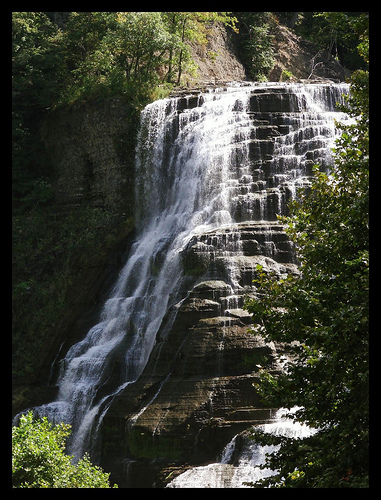
\includegraphics[height=1in]{imggrid/datasetposi/2.jpg} &
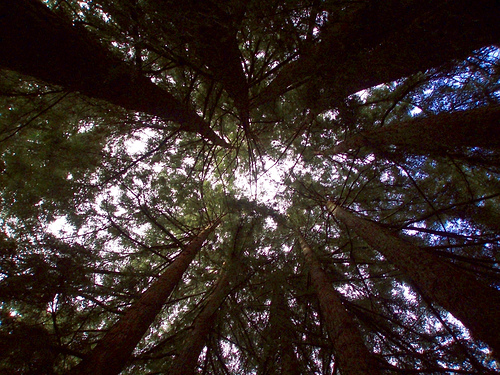
\includegraphics[width=0.19\textwidth]{imggrid/datasetposi/3.jpg} &
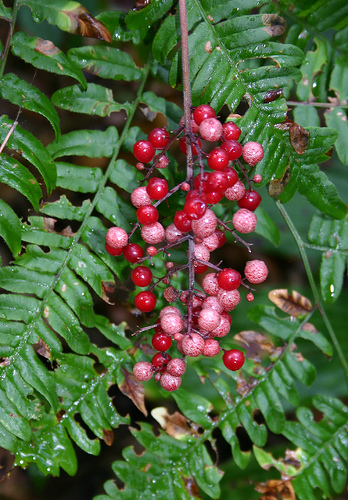
\includegraphics[height=1in]{imggrid/datasetposi/4.jpg} &
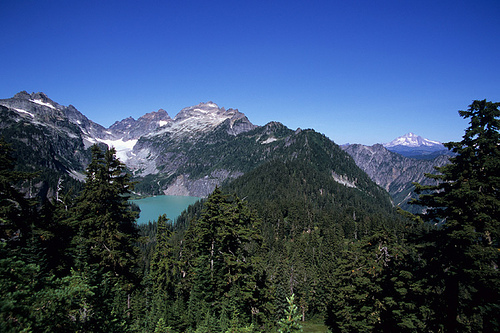
\includegraphics[width=0.19\textwidth]{imggrid/datasetposi/5.jpg} \\
%\multicolumn{5}{c}{(a) Random positive images in vegetation dataset} \\
\\[-6pt]
\hline
\\[-6pt]
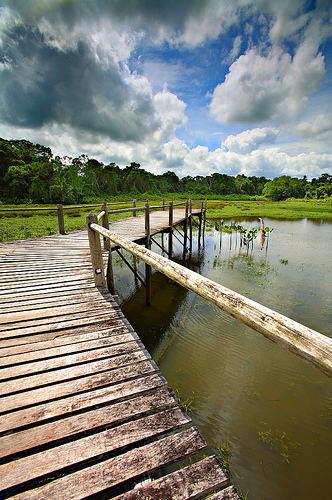
\includegraphics[height=1in]{imggrid/datasetposi/6.jpg} &
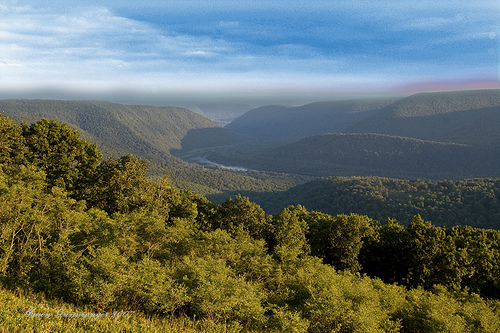
\includegraphics[width=0.19\textwidth]{imggrid/datasetposi/7.jpg} &
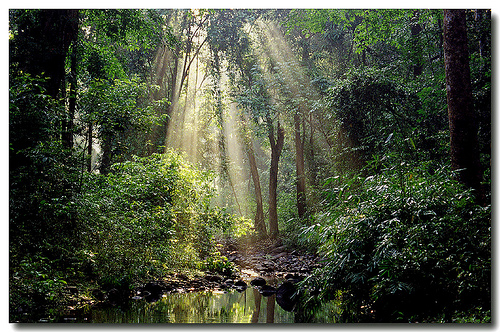
\includegraphics[width=0.19\textwidth]{imggrid/datasetposi/8.jpg} &
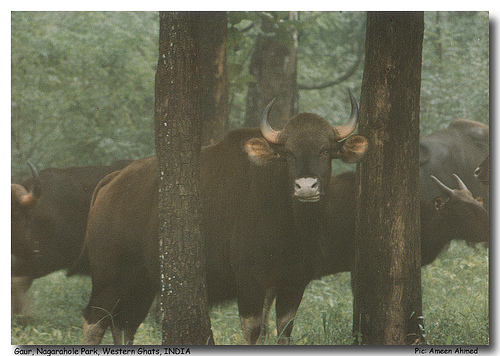
\includegraphics[width=0.19\textwidth]{imggrid/datasetposi/9.jpg} &
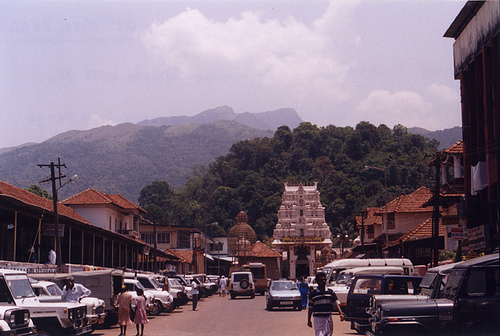
\includegraphics[width=0.19\textwidth]{imggrid/datasetposi/10.jpg} \\
\multicolumn{5}{c}{(a) Random positive images in vegetation dataset} \\ 
\\[-6pt]
\hline
\\[-6pt]
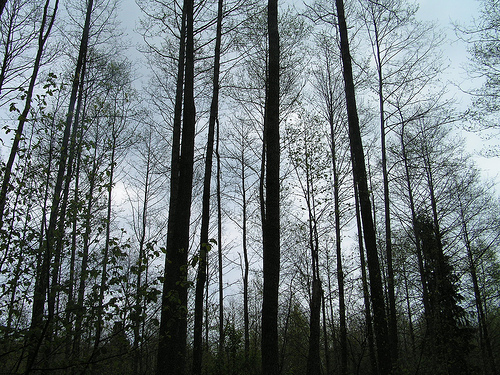
\includegraphics[width=0.19\textwidth]{imggrid/datasetnega/1.jpg} &
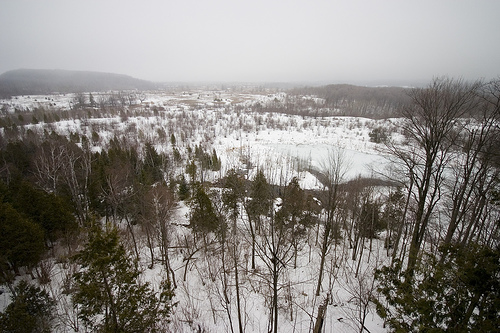
\includegraphics[width=0.19\textwidth]{imggrid/datasetnega/2.jpg} &
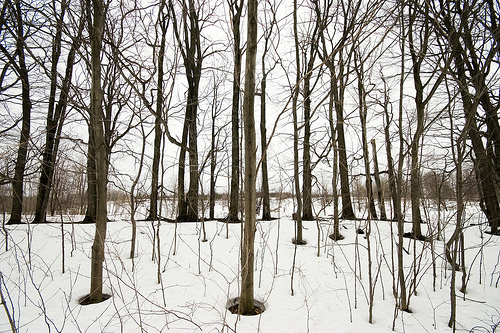
\includegraphics[width=0.19\textwidth]{imggrid/datasetnega/3.jpg} &
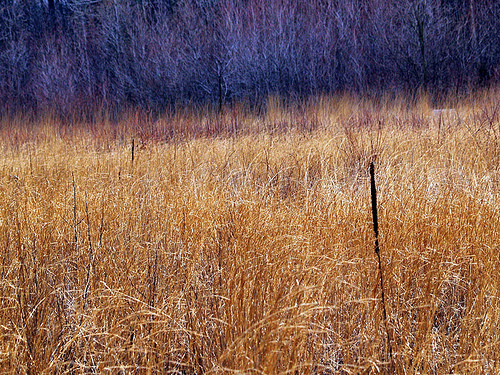
\includegraphics[width=0.19\textwidth]{imggrid/datasetnega/4.jpg} &
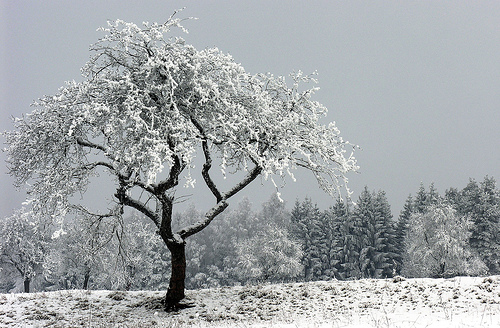
\includegraphics[width=0.19\textwidth]{imggrid/datasetnega/5.jpg} \\
%\multicolumn{5}{c}{(c) Random false negatives (snow images classified as non-snow)} \\ 
\\[-6pt]
\hline
\\[-6pt]
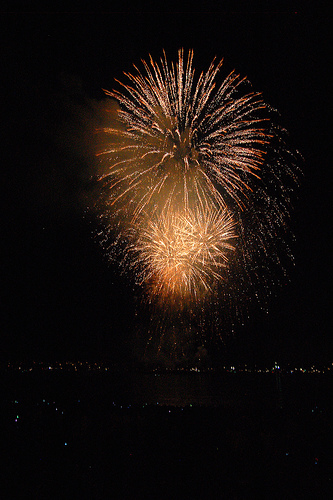
\includegraphics[height=1in]{imggrid/datasetnega/6.jpg} &
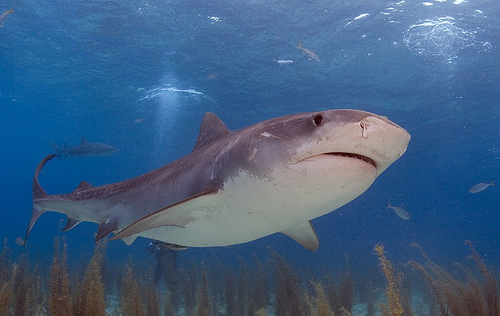
\includegraphics[width=0.19\textwidth]{imggrid/datasetnega/7.jpg} &
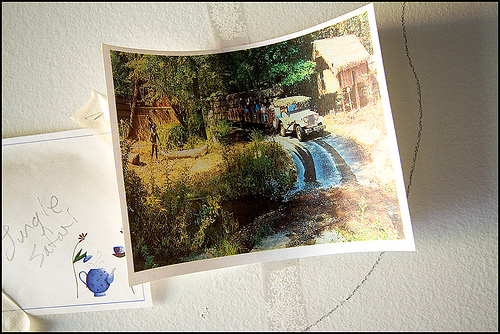
\includegraphics[width=0.19\textwidth]{imggrid/datasetnega/8.jpg} &
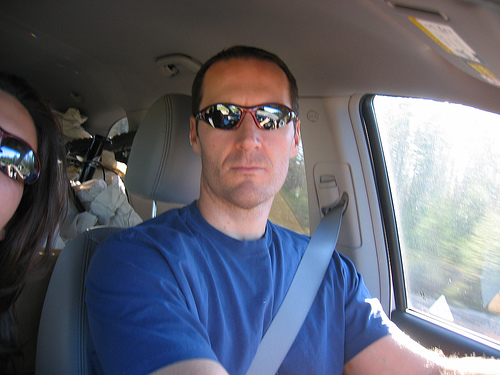
\includegraphics[width=0.19\textwidth]{imggrid/datasetnega/9.jpg} &
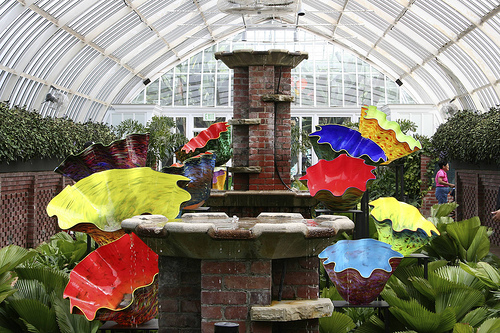
\includegraphics[width=0.19\textwidth]{imggrid/datasetnega/10.jpg} \\
\multicolumn{5}{c}{(b) Random negative images in vegetation dataset} \\
\end{tabular}
\end{center}
}}
\caption{Random images from our hand-labeled dataset. Public sharing images are various in quality, contents, illumination and view angle.
Negative images like winter trees without leaves, or indoor images capturing a photo of forest are more confusing.}
\label{fig:dataset}
\end{figure*}


\end{document}